\documentclass{beamer}
\usefonttheme{professionalfonts}
%\usetheme{Rochester}
%\usetheme{AnnArbor}
\usetheme{Szeged}
\useoutertheme{infolines}
\usecolortheme{dolphin}
\usepackage{graphicx}
% \usepackage[english]{babel}
\usepackage{hyperref}
\usepackage{multicol}
\usepackage{color}
%\usepackage{smartdiagram}


%\definecolor{carmine}{rgb}{0.59, 0.0, 0.09}
\usepackage{amsmath} 

\usepackage{graphicx}
\usepackage{tikz}
\usetikzlibrary{shapes.callouts}
\usepackage{multirow}

\usepackage[utf8]{inputenc}

\usepackage{enumerate}
\usepackage[shortlabels]{enumitem}
\usepackage{amsmath,amsthm,amssymb,amsfonts,mathrsfs,latexsym,stmaryrd}
\usepackage{tcolorbox}

\usepackage{color} 
\usepackage{amssymb, amsmath, amsbsy}
\usepackage{adjustbox,lipsum}
\usepackage{placeins}

\usepackage{textpos}
\usepackage{wrapfig}
\usepackage[spanish, es-tabla]{babel}

\usepackage{caption}
\setlength{\parindent}{15pt}
% Beamer already loads hyperref; avoid reloading it with conflicting options.

\usepackage{url}
\usepackage{float}
\usepackage{tikz}
\usetikzlibrary{patterns}


\title{ Repaso ayudantía}

\author{Francisco Alfaro Medina}
\institute[USM]
{Universidad Técnica Federico Santa María\\ % Your institution for the title page
	\medskip
	\textit{} % Your email address
	
}
\logo{

\includegraphics[width=1cm]{../Imagenes/Logo_UTFSM.png}
}
\date{}
\newcommand\Fontvi{\fontsize{9}{7.2}\selectfont}
\begin{document}
	
\begin{frame}
	\titlepage % Print the title page as the first slide
\end{frame}
	
\section{Estadística}


\begin{frame}
\frametitle{Ramas de la  Estadística }
La Estadística se divide en dos
áreas:

\begin{itemize}
\item\textbf{{\color{blue} Estadística Descriptiva:}} se emplea como una primera aproximación a los datos. Utiliza tablas y gráficos para resumir la información disponible.
\item \textbf{{\color{blue} Estadística Inferencial:}} va un poco más allá. A partir de los datos desarrolla mecanismos de decisión parar determinar si los datos sustentan o no una hipótesis. Permite hacer predicciones. 
\end{itemize}

\end{frame}


%------------------------------------------------------------------------------------------------------------------------------------------------
%------------------------------------------------------------------------------------------------------------------------------------------------

\begin{frame}
\frametitle{ Estadística Descriptiva}

\begin{itemize}
\item Los \textbf{{\color{blue}estadísticos}} son funciones de los datos de una muestra:
$$f(X_1,....,X_n)$$
\item \textbf{gráficos}: histogramas, gráficos de caja
\item \textbf{tablas}: de frecuencia, contingencia, etc.
\end{itemize}
\end{frame}


%------------------------------------------------------------------------------------------------------------------------------------------------
%------------------------------------------------------------------------------------------------------------------------------------------------


\begin{frame}
\frametitle{Estadísticos de Localización  Central}

\begin{itemize}
\item \textbf{{\color{blue}Media empírica o promedio}}:
$$\bar{X}=\frac{1}{n}\sum_{i=1}^n X_i$$


\item \textbf{{\color{blue}Mediana}}: Si se tiene una muestra $X_1,...,X_n$, se ordenan los datos de menor a mayor:
$X_{(1)},...X_{(n)}$. La mediana es la observación que queda en el
medio.

$$Med(X_1,....,X_n)=\left\{
                      \begin{array}{ll}
                        X_{(\frac{n+1}{2})}, & \hbox{si $n$ es impar} \\
                        \frac{X_{(n/2)}+X_{(n/2+1)}}{2}, & \hbox{si $n$ es par}
                      \end{array}
                    \right.
$$
\end{itemize}
\end{frame}

%------------------------------------------------------------------------------------------------------------------------------------------------
%------------------------------------------------------------------------------------------------------------------------------------------------




%------------------------------------------------------------------------------------------------------------------------------------------------
%------------------------------------------------------------------------------------------------------------------------------------------------


\begin{frame}
\frametitle{Estadísticos de Localización  Central}

\begin{itemize}
\item Suponiendo que se tienen 13 datos (caso de $n$ impar): $$X_{(1)},......,\underbrace{X_{(7)}}_\text{mediana},......,X_{(13)}$$

\item Suponiendo que se tienen 12 datos (caso de $n$ par): $$X_{(1)},......,\underbrace{X_{(6)},X_{(7)}}_\text{mediana$=\frac{X_{(6)}+X_{(7)}}{2}$},......,X_{(12)}$$
% \item A la mediana se la conoce también como \textbf{percentil} 50. El 50\% de los datos son menores que la mediana
\end{itemize}
\end{frame}


%------------------------------------------------------------------------------------------------------------------------------------------------
%------------------------------------------------------------------------------------------------------------------------------------------------




%------------------------------------------------------------------------------------------------------------------------------------------------
%------------------------------------------------------------------------------------------------------------------------------------------------

% \begin{frame}
% \frametitle{Estadísticos de  Localización}

% \begin{itemize}
% \item Un percentil es una medida estadística que indica la posición de un dato dentro de un conjunto de observaciones, dividiendo los datos en 100 partes iguales.

% \item La fórmula para calcular el \textbf{\textit{percentil de $a$ porciento }} $P_{a}$, con $0<a<100$  es:\\
% $$ P_{a}(x_1,...,x_n)=
%     \left\{
%     \begin{array}{ll}
%         x_{(y_a+1)}, & \hbox{si $y_a=[y_a]$} \\
%         \frac{x_{([y_a])}+ x_{([y_a]+1)}}{2}, & \hbox{si $y_a>[y_a]$}
%     \end{array}
%     \right.
% $$\\

% donde $y_a=\frac{an}{100}$, e $[y_a]$ es la parte entera de $y_a$

% \end{itemize}

% \end{frame}

%------------------------------------------------------------------------------------------------------------------------------------------------
%------------------------------------------------------------------------------------------------------------------------------------------------

\begin{frame}
\frametitle{Estadísticos de  Localización}

\begin{itemize}
\item Un percentil es una medida estadística que indica la posición de un dato dentro de un conjunto de observaciones, dividiendo los datos en 100 partes iguales.
\item Los percentiles más empleados son: $P_{25}$, $P_{50}=Mediana$, $P_{75}$ y se conocen como \textbf{\textit{{\color{blue}cuartiles}}}
ya que dividen a los datos en 4 partes (se suelen nombrar $q_1$, $q_2$ y
 $q_3$).
\item También existen los \textbf{{\color{blue}quintiles} }y \textbf{{\color{blue}deciles}}, según se dividan a los datos en 5 o 10 partes.
\end{itemize}

\end{frame}

%------------------------------------------------------------------------------------------------------------------------------------------------
%------------------------------------------------------------------------------------------------------------------------------------------------

% \begin{frame}
% \frametitle{ESTADÍSTICOS DE DISPERSIÓN}



%   \begin{figure}[ht]
%    \centering
%    \subfigure{
%    {\includegraphics[width=5cm]{graficos/clase1_disp1}}
%    }
%    \subfigure{
%    {\includegraphics[width=5cm]{graficos/clase1_disp2}}
%    }
%    \end{figure}

% \end{frame}


%------------------------------------------------------------------------------------------------------------------------------------------------
%------------------------------------------------------------------------------------------------------------------------------------------------

\begin{frame}
\frametitle{Estadísticos de dispersión }

\begin{itemize}
\item El \textit{\textbf{rango intercuartílico}}: se define como: \[RIQ(X_1,...,X_n)=q_3-q_1\]
\item La \textit{\textbf{varianza muestral o empírica}} se define como:
\[Var(X_1,...,X_n)=\frac{\sum_{i=1}^n (X_i-\bar{X})^2}{n-1}\]
\end{itemize}

\end{frame}


%------------------------------------------------------------------------------------------------------------------------------------------------
%------------------------------------------------------------------------------------------------------------------------------------------------


\begin{frame}
 \frametitle{Estadísticos de dispersión }

 \begin{itemize}
\item La \textit{\textbf{{\color{blue}desviación estándar muestral o empírico}}} es la raíz cuadrada de la varianza, es decir:
 \[S(X_1,...,X_n)=\sqrt{\frac{\sum_{i=1}^n (X_i-\bar{X})^2}{n-1}}\]
% \item \emph{\textbf{{\color{blue}coeficiente de variación de Pearson}}}: se define como
% \[ CV(X_1,....,X_n)=\frac{S}{\bar{X}}.\]
% También se puede expresar en forma porcentual:
% \[ CV(X_1,....,X_n)=\frac{S}{\bar{X}}100\]
 \end{itemize}

\end{frame}


%------------------------------------------------------------------------------------------------------------------------------------------------
%------------------------------------------------------------------------------------------------------------------------------------------------

  \begin{frame}{ Histograma}
      El histograma resume los datos dentro de algunos rangos y se cuenta el número de observaciones dentro de cada rango.

     \begin{figure}
         \centering
         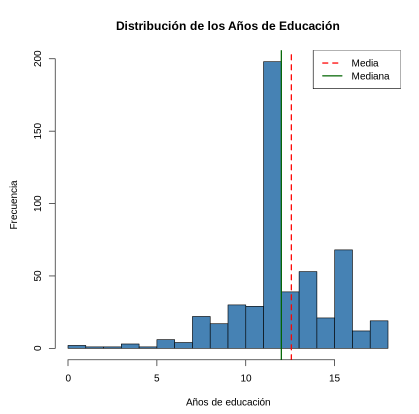
\includegraphics[width=0.5\linewidth]{../Imagenes/hist.png}
     \end{figure}

     \href{https://colab.research.google.com/drive/1fGx_sLiasa-psVeudjO5IgJPPJX0lB6t?usp=sharing}{\beamergotobutton{Colab}}
        
  \end{frame}

 

  
\begin{frame}
\frametitle{Gráfico de caja - Boxplot}


\begin{figure}
    \centering
    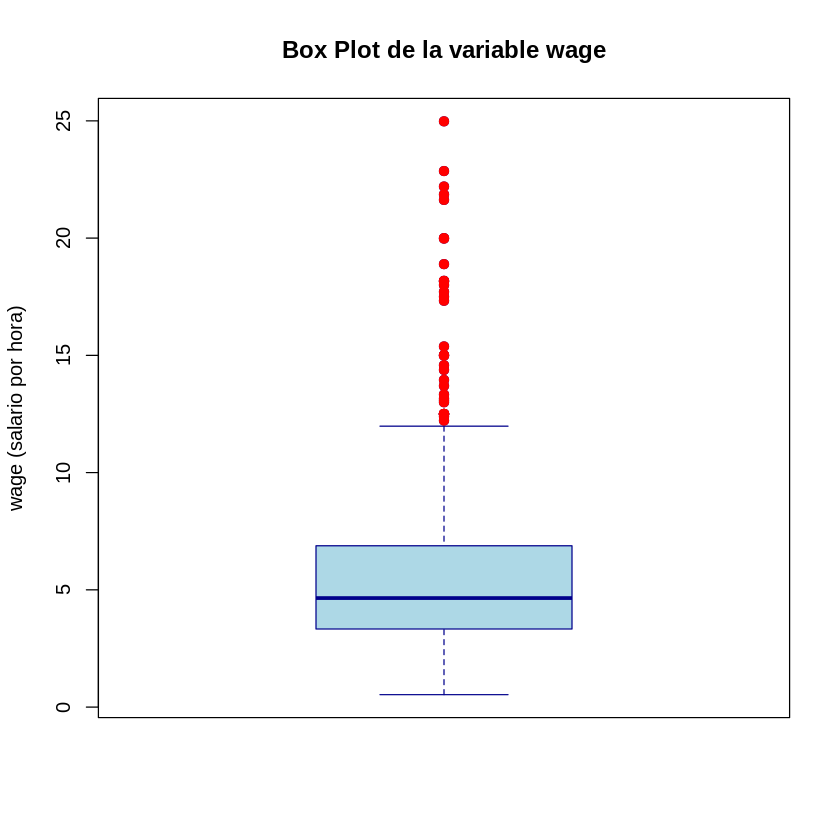
\includegraphics[width=0.62\linewidth]{box_plot.png}
\end{figure}


\end{frame}

%------------------------------------------------------------------------------------------------------------------------------------------------
%------------------------------------------------------------------------------------------------------------------------------------------------


\begin{frame}
\frametitle{Gráfico de caja - Boxplot}
\begin{itemize}

\item \underline{\textit{Línea en medio de la caja}}: $Med$ (mediana).
\item \underline{\textit{Límite superior de la caja}}: $q_3$ (tercer cuartil).
\item \underline{\textit{Límite inferior de la caja}}: $q_1$ (primer cuartil).
\item notar que el largo de la caja representa el $RIQ$ (rango intercuartilico).
\item \underline{\textit{Bigote superior}}: es el mínimo entre $ q_3+ 1.5RIQ$ y el máximo de los datos ($X_n$).
\item \underline{\textit{Bigote inferior}}: es el máximo entre $q_1 - 1.5RIQ$ y el mínimo de los datos ($X_1$).
\item \underline{\textit{Puntos fuera de los bigotes}}: Todos los puntos que exceden los bigotes se grafican. Son puntos extremos (atípicos).
\end{itemize}
\end{frame}

%------------------------------------------------------------------------------------------------------------------------------------------------
%------------------------------------------------------------------------------------------------------------------------------------------------


 
%  \begin{frame}{}
     
%  \end{frame}
\end{document}
